\subsection{Use-case gợi ý món ăn (Food Suggestion)}
    \begin{figure}[h]
        \centering
        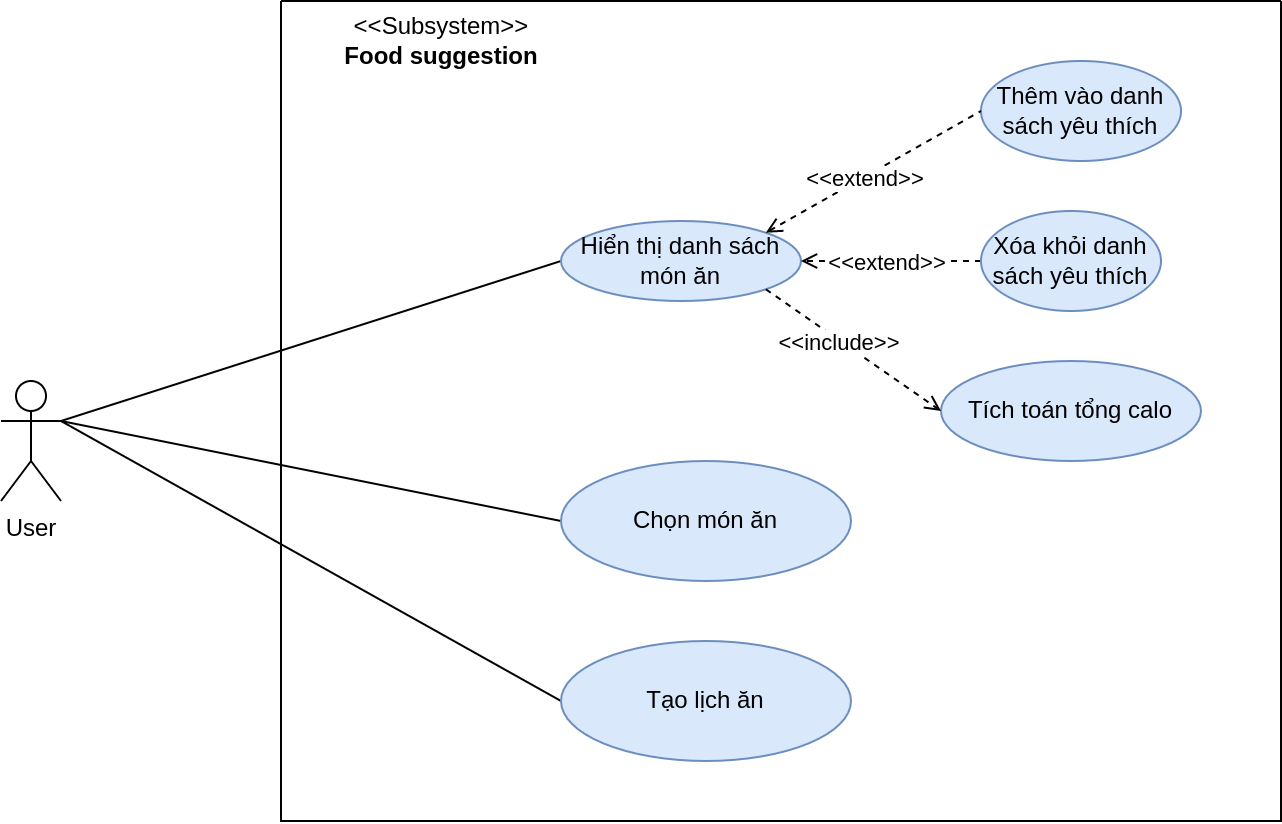
\includegraphics[width=1\linewidth]{images/use-case diagram/food-suggestion_use-case.png}
        \caption{Use-case gợi ý món ăn}
    \end{figure}
    
    \begin{tblr}{
        width=1\linewidth,
        hlines,
        vlines,
        colspec={X[3]X[7]},
        columns = {valign = m, },
        row{1} = {halign = c, valign = m, bg = lightgray, fg = black},
    }
        {\textbf{Use case name} & \textbf{Hiển thị danh sách món ăn}}  \\
        Description	 & 	Hệ thống hiển thị danh sách các món ăn \\
        Actor & Người dùng (User) \\
        Trigger & 	Người dùng ấn vào nút tạo lịch ăn trong ngày \\
        Pre-condition & Người dùng đã đăng nhập vào hệ thống\\
        Post-condition & Các món ăn được hiển thị trên màn hình\\
        Normal flow &   1. Người dùng chọn vào tạo lịch ăn \newline
                    	2. Hệ thống truy cập vào database \newline
                    	3. Hệ thống tính toán tổng lượng calo phù hợp \newline 
                    	4. Hệ thống hiển thị các món ăn \\
        Alternative flow  & Alternative flow thứ 1: tại bước 1 \newline
                        	1a Người dùng ấn vào thêm món ăn trong lịch ăn đã có sẵn \newline
                        	Use case tiếp tục bước 2 \newline
                        	\newline
                        	Alternative flow thứ 2: tại bước 1 \newline
                        	2a Người dùng chọn vào phần các món ăn ưa thích \newline
                        	2b Hệ thống truy cập vào các món ăn ưu thích của người dùng \newline
                        	Use case tiếp tục bước 3\\
        Exception flow & 	Exception flow thứ 1: tại bước 3 \newline
                            1a Nếu không có món ăn phù hợp, báo lỗi không có món ăn phù hợp \\
       Extended points & Thêm vào danh sách ưa thích, loại khỏi dánh sách ưa thích
    \end{tblr}
    
    \begin{tblr}{
        width=1\linewidth,
        hlines,
        vlines,
        colspec={X[3]X[7]},
        columns = {valign = m, },
        row{1} = {halign = c, valign = m, bg = lightgray, fg = black},
    }
        {\textbf{Use case name} & \textbf{Thêm vào danh sách ưa thích}}  \\
        Description	& Người dùng thêm món ăn vào danh sách ưu thích \\
        Actor & Người dùng (User) \\
        Trigger & Người dùng ấn nút thêm vào danh sách yêu thích  \\
        Pre-condition & Người dùng đang ở danh sách các món ăn\\
        Post-condition & Món ăn được thêm vào danh sách yêu thích\\
        Normal flow &   		1. Người dùng chọn vào món ăn \newline
                                2. Hệ thống hiển thị chi tiết món ăn \newline
                            	3. Người dùng ấn vào nút trái tim \newline 
                            	4. Hệ thống lưu lại món ăn mà người dùng thích \\
        Alternative flow  & 	Alternative flow thứ 1: tại bước 1 \newline
                            	1a Người dùng ấn vào nút 3 chấm ở 1 món ăn trong danh sách các món ăn \newline 
                            	1b Hê thống hiện thị các tùy chọn \newline
                            	1c Người dùng ân vào dòng thêm vào mục ưa thích \newline
                            	Use case tiếp tục bước 3 \\
        Exception flow & none\\
    \end{tblr}
    
    \vspace{0.7cm}
    
    \begin{tblr}{
        width=1\linewidth,
        hlines,
        vlines,
        colspec={X[3]X[7]},
        columns = {valign = m, },
        row{1} = {halign = c, valign = m, bg = lightgray, fg = black},
    }
        {\textbf{Use case name} & \textbf{Xóa khỏi danh sách ưa thích}}  \\
        Description	& Xóa món ăn khỏi danh mục ưa thích \\
        Actor & Người dùng (User) \\
        Trigger & Người dùng ấn vào nút xóa khỏi danh sách ưa thích  \\
        Pre-condition & Người dùng đang ở danh sách các món ăn\\
        Post-condition & Món ăn được thêm vào danh sách yêu thích\\
        Normal flow &   	1. Người dùng chọn món ăn \newline
                            2. Hệ thống hiển thị chi tiết  món ăn \newline
                            3. Người dùng ấn nút loại bỏ khỏi danh sách \newline
                            4. Hệ thống ghi nhận xóa món ăn khỏi danh sách ưa thích\\
        Alternative flow  & 	Alternative flow thứ 1: Tại bước 1 \newline
                            	1a. Người dùng ấn vào nút 3 chấm \newline
                            	1b. Người dùng chọn xóa khỏi danh sách ưa thích \newline
                            	Tiếp tục bước 4\\
        Exception flow & none\\
    \end{tblr}
    
    \vspace{0.7cm}
    
    \begin{tblr}{
        width=1\linewidth,
        hlines,
        vlines,
        colspec={X[3]X[7]},
        columns = {valign = m, },
        row{1} = {halign = c, valign = m, bg = lightgray, fg = black},
    }
        {\textbf{Use case name} & \textbf{Chọn món ăn}}  \\
        Description	& Người dùng chọn món ăn cho vào lịch ăn \\
        Actor & Người dùng (User) \\
        Trigger & Người ấn vào nút thêm món ăn \\
        Pre-condition & Người dùng đang ở trang danh sách món ăn\\
        Post-condition & Món ăn được thêm vào lịch ăn\\
        Normal flow &   	1. Người dùng chọn thêm món ăn trên danh sách \newline
                            2. Món ăn được chọn đươc lưu vào lịch ăn \\
        Alternative flow  & none\\
        Exception flow & none\\
    \end{tblr}

    \begin{tblr}{
        width=1\linewidth,
        hlines,
        vlines,
        colspec={X[3]X[7]},
        columns = {valign = m, },
        row{1} = {halign = c, valign = m, bg = lightgray, fg = black},
    }
        {\textbf{Use case name} & \textbf{Tạo lịch ăn}}  \\
        Description	& Người dùng chọn món ăn cho vào lịch ăn \\
        Actor & Người dùng (User) \\
        Trigger & Người dùng ấn vào giỏ các món ăn đã chọn \\
        Pre-condition & 	Người dùng đã có các món ăn được chọn\\
        Post-condition & 	Lịch ăn được tạo thành công\\
        Normal flow &   	1. Người dùng bấm vào giỏ xem các món ăn đã chọn \newline
                        	2. Người dùng bấm nút tạo lịch ăn \newline
                        	3. Hệ thống lưu lại lịch ăn đã được người dùng chọn \newline
                        	4. Hệ thống gửi thông báo xác nhận lịch ăn được tạo thành công\\
        Alternative flow  & none\\
        Exception flow & none\\
    \end{tblr}

\newpage